
\documentclass[conference]{IEEEtran}


\usepackage{cite}
\usepackage[pdftex]{graphicx}
\usepackage[cmex10]{amsmath}
\usepackage{amsfonts}
\usepackage{algorithmic}
\usepackage{array}
\usepackage{mdwmath}
\usepackage{mdwtab}
%\usepackage{eqparbox}
\usepackage[caption=false,font=footnotesize]{subfig}
\usepackage{fixltx2e}
\usepackage{url}
\usepackage{color}


\interdisplaylinepenalty=1000

\newenvironment{meta}[0]{\color{red} \em}{}

% correct bad hyphenation here
\hyphenation{}



\begin{document}



\title{Variable Rate Models for Tracking}

\author{
\IEEEauthorblockN{Pete Bunch\\ and Simon Godsill}
\IEEEauthorblockA{Signal Processing and Communications Laboratory\\
Cambridge University Engineering Dept., UK\\
Email: \{pb404, sjg30\}@eng.cam.ac.uk}
}

\maketitle



\begin{abstract}

The problem of tracking moving targets is often handled by modelling using hidden Markov models. This approach is attractive because it allows standard algorithms to be used, including the Kalman filter and particle filter. However, it often ignores a significant amount of temporal structure in the path of a manoeuvring target. Variable rate models treat the target motion as deterministic when conditioned upon a sequence of changepoint times and manoeuvre parameters. In this paper, new variable rate models for tracking are presented. Previously, a 2-dimensional model has been developed which parameterises the motion with tangential and normal accelerations. This model is improved by introducing additional variables to improve resilience to model error. It is then modified for use in 3 dimensions by assuming manoeuvres are planar. Simulation tests demonstrate improved tracking performance on a benchmark aeroplane trajectory.

\end{abstract}



\section{Introduction}

Tracking is the task of inferring kinematic state of a target (position, velocity, etc.) over time from a set noisy or partial observations. The state of the target is a continuous process and is likely to be highly structured. However, many tracking systems model target dynamics as a discrete-time Markov process \cite{Li2003}. This assumption has the advantage of simplicity --- by discretising the state at observation times, we arrive at a hidden Markov model, with which standard Kalman \cite{Anderson1979} or particle \cite{Cappe2007,Doucet2009} filtering and smoothing methods may be used. The disadvantage of such an assumption is that it may be a poor reflection of the system dynamics, disregarding long-term temporal structure in the state trajectory.

Recently, variable rate models have been developed for tracking, \cite{Godsill2007a,Godsill2007,Whiteley2011}. These models treat the kinematic state as a continuous process which is deterministic conditional upon an underlying sequence of changepoint times and motion parameters. This underlying changepoint sequence may be considered to be a realisation of a marked point process (MPP), with the resulting state trajectory as a piecewise-deterministic process (PDP). (The relationship between MPPs and PDPs is explored thoroughly in \cite{Jacobsen2006}, along with a rigorous description of associated probability measures.) The sequence of changepoints may be estimated numerically, using a variable rate particle filter, leading to a particle approximation of the current posterior state distribution.

In a tracking scenario, changepoints represent the beginning and end of target manoeuvres, each of which is governed by an associated parameter vector (e.g. accelerations). In \cite{Whiteley2011}, a 2-dimensional (2D) dynamic model is considered in which the accelerations along the Cartesian axes are fixed for the duration of each manoeuvre. In \cite{Godsill2007}, a variation is used in which the target experiences tangential and normal accelerations whose magnitudes are fixed throughout each manoeuvre, but whose directions are specified relative to the target velocity. This intrinsic coordinate model is more complex but also more realistic -- the two components can be thought of as throttle and steering controls.

These variable rate tracking models suffer from a lack of degrees of freedom. Both the Cartesian and intrinsic versions have four state variables (two position, two velocity), but only two governing accelerations. The result is that from a given manoeuvre start point, it is not possible to reach every combination of state variables. This can lead to poor tracking performance, especially if the state is fully observed (for example, using radar with Doppler measurements of velocity).

In this paper, we present extensions to the intrinsic coordinate tracking model for use with variable rate particle filtering and smoothing algorithms. First, an augmented version of the 2D model is outlined which addresses the problem of under-parametrisation. Secondly, 3-dimensional (3D) extensions of the 2D model are discussed for manoeuvring aircraft.



\section{Variable Rate Particle Filter}

The main focus of this paper is the development of dynamics models for variable rate systems, so only a brief overview of the variable rate particle filter is included here, to motivate the following sections. For a more detailed exposition, see \cite{Godsill2007a,Godsill2007,Whiteley2011}.

We consider a general model from time $0$ to $T$, between which observations, $\{y_1 \dots y_N\}$, are made at times $\{t_1 \dots t_N = T\}$. During this period, an unknown number of changepoints, $K$, occur at times $\{\tau_0 = 0, \tau_1 \dots \tau_K \}$, each with associated changepoint parameters, $\{ u_0, u_1 \dots u_K \}$. The pairs $\{\tau_k, u_k\}$ are the elements of an marked point process (MPP). The latent state is a continuous-time process denoted $x(t)$. Discrete sets containing multiple values over time will be written as, e.g. $y_{1:n} = \{y_1 \dots y_n\}$.

The objective for inference will be to estimate the changepoint sequence up until the current time $\theta_n = \{\tau_{j}, u_{j} \forall j : 0 \leq \tau_j < t_n \}$. It will also be useful to define a variable for the changepoints which occur in the interval $[t_{n-1},t_n)$, $\theta_{n \setminus n-1} = \{\tau_{j}, u_{j} \forall j : t_{n-1} \leq \tau_j < t_n \}$.

For notational simplicity, the following counting variables are introduced to keep track of the most recent changepoint to have occurred,
%
\begin{IEEEeqnarray}{rCl}
 K(t)  & = & \max(k : \tau_k<t) \\
 K_n   & = & K(t_n)     .
\end{IEEEeqnarray}

The changepoint sequence is assumed to be a Markov process,
%
\begin{IEEEeqnarray}{rCl}
 \{\tau_k, u_k\} & \sim & p(u_k|\tau_k, \tau_{k-1}, u_{k-1}) p(\tau_k|\tau_{k-1}, u_{k-1}) \label{eq:cp_model}     .
\end{IEEEeqnarray}

From this, a prior density for the changepoint sequence, $p(\theta_n)$ and the sequence extension $p(\theta_{n \setminus n-1})$ may be written down. See \cite{Jacobsen2006,Whiteley2011} for details.

The state dynamics will be governed by a differential equation depending upon the most recent changepoint.
%
\begin{IEEEeqnarray}{rCl}
 dx(t) & = & \mathrm{f}(x(t), \tau_{K(t)}, u_{K(t)}) \label{eq:state_differential_eq}     .
\end{IEEEeqnarray}

By introducing a new sequence, $\{ x_0, x_1 \dots x_K \}$, which denotes the value of the state at each changepoint (i.e. $x(\tau_k)$), and assuming that an analytic solution exists, a state transition function may be found,
%
\begin{IEEEeqnarray}{rCll}
 x(t) & = & f(x_{K_n}, v_{K_n}, \tau_{K_n}, t) &, \tau_{K_n} \leq t \leq \tau_{K_{n}+1} \label{eq:disc_time_state_trans_func}     .
\end{IEEEeqnarray}

By choosing $t = \tau_{K_{n}+1}$, this equation specifies the state at the next changepoint time. Similarly, by choosing $t=t_n$, the state at the observation times may be calculated. These points will be denoted $\hat{x}_n$. To complete the model, a probabilistic measurement model must be chosen for the observation process, $p(y_n|\hat{x}_n)$.

The variable rate particle filter (VRPF) sequentially estimates the following changepoint posterior distribution,
%
\begin{IEEEeqnarray}{rCl}
\IEEEeqnarraymulticol{3}{l}{p(\theta_{n}|y_{1:n})} \nonumber \\
 & \propto & p(y_n|\theta_{n}, y_{1:n-1}) p(\theta_{n \setminus n-1}|\theta_{n-1}) p(\theta_{n-1}|y_{1:n-1}) \label{eq:vrpf_target}     .
\end{IEEEeqnarray}

Each particle in the approximation is a sequence of changepoints between $0$ and $t_n$. A particle is generated by proposing from the importance distribution,
%
\begin{equation}
 q(\theta_{n}) = \sum_j v_{n-1}^{(j)} \delta_{\theta_{n-1}^{(j)}}(\theta_{n-1}) q(\theta_{n \setminus n-1}|\theta_{n-1}, y_n).
\end{equation}

The resampling weights $v_{n-1}^{(j)}$ are chosen appropriately to achieve no resampling, normal resampling or auxiliary resampling.

The particle is then weighted according to the ratio of target and proposal densities,
%
\begin{IEEEeqnarray}{rCl}
w_n^{(i)} & = & \frac{ p(\theta_{n}^{(i)}|y_{1:n}) }{ q(\theta_{n}^{(i)}) } \nonumber \\
    & =       & \frac{w_{n-1}^{(i)}}{v_{n-1}^{(i)}} \times \frac{ p(y_n|\hat{x}_n) p(\theta_{n \setminus n-1}|\theta_{n-1}) }{ q(\theta_{n \setminus n-1}|\theta_{n-1}^{(i)}, y_n) } \label{eq:vrpf_weights}
\end{IEEEeqnarray}

The normalisation may be enforced by scaling the weights so that they sum to $1$.

For the bootstrap VRPF, the sequence extension transition density is used as the proposal, $q(\theta_{n \setminus n-1}|\theta_{n-1}, y_n) = p(\theta_{n \setminus n-1}|\theta_{n-1})$, resulting in the usual simplification of the importance weights.

Filter performance may be improved by allowing previously proposed changepoints to be modified, either by adding resample-move steps \cite{Gilks2001}, or by using the sequential Monte Carlo sampler method of \cite{Whiteley2011}.

The rest of the paper is concerned with suitable choices for the state differential equation (\ref{eq:state_differential_eq}) and the resulting form of the transition function (\ref{eq:disc_time_state_trans_func}).



\section{2D Intrinsic Coordinate Model}

For the simplest 2D intrinsic coordinate model, the target is treated as a particle subject to two accelerations, one tangential, $a_{T,k}$, and one normal, $a_{N,k}$, to the current velocity. The accelerations are fixed for the duration of a manoeuvre. The continuous-time kinematic state of the target is described by the bearing, $\psi(t)$ (anticlockwise relative to the $x$ axis), and speed $\dot{s}(t)$, as well as the Cartesian coordinates, $x(t)$ and $y(t)$.

Thus, the state and parameter vectors are,
%
\begin{IEEEeqnarray}{rCl}
\mathbf{x}(t) & = & [ x(t), y(t), \psi(t), \dot{s}(t) ]^T \\
\mathbf{u}_k  & = & [ a_{T,k}, a_{N,k} ]^T
\end{IEEEeqnarray}

The target dynamics are described by the following standard differential equations for curvilinear motion,
%
\begin{IEEEeqnarray}{rCl}
\ddot{s}_t & = & a_{T,K(t)} \label{eq:aT_ode} \\
\dot{s}_t \dot{\psi}_t & = & a_{N,K(t)} \\
\dot{x}_t & = & \dot{s}_t \cos(\psi_t) \\
\dot{y}_t & = & \dot{s}_t \sin(\psi_t)     .
\end{IEEEeqnarray}

Solving this system of equations yields the following state transition function, where $\Delta t = t - \tau_{K(t)}$,
%
\begin{IEEEeqnarray}{rCl}
\dot{s}(t) & = & \dot{s}_{K(t)} + a_{T,k} \Delta t \label{eq:2D_ICmodel_start} \\
\psi(t) & = & \psi_{K(t)} + \frac{a_{N,k}}{a_{T,k}} \log \left( \frac{\dot{s}(t)}{\dot{s}_{K(t)}} \right) \\
x(t) & = & x_{K(t)} \\
     \IEEEeqnarraymulticol{3}{l}{ \quad + \: \frac{ \dot{s}(t)^2 }{ 4 a_{T,k}^2 + a_{N,k}^2 } \left[  a_{N,k} \sin(\psi(t)) + 2 a_{T,k} \cos(\psi(t))  \right]} \nonumber \\
     \IEEEeqnarraymulticol{3}{l}{ \quad - \: \frac{\dot{s}_{K(t)}^2}{4 a_{T,k}^2 + a_{N,k}^2} \left[  a_{N,k} \sin(\psi_{K(t)}) + 2 a_{T,k} \cos(\psi_{K(t)})  \right]} \nonumber \\
y(t) & = & y_{K(t)} \label{eq:2D_ICmodel_stop} \\
     \IEEEeqnarraymulticol{3}{l}{ \quad + \: \frac{ \dot{s}(t)^2 }{ 4 a_{T,k}^2 + a_{N,k}^2 } \left[ -a_{N,k} \cos(\psi(t)) + 2 a_{T,k} \sin(\psi(t))  \right]} \nonumber \\
     \IEEEeqnarraymulticol{3}{l}{ \quad - \: \frac{\dot{s}_{K(t)}^2}{4 a_{T,k}^2 + a_{N,k}^2} \left[  -a_{N,k} \cos(\psi_{K(t)}) + 2 a_{T,k} \sin(\psi_{K(t)})  \right]} \nonumber      .
\end{IEEEeqnarray}

Particular care must be taken when $a_{T,k} \rightarrow 0$ or $a_{N,k} \rightarrow 0$ (or both). These cases can be handled using L'H\^{o}pital's rule or by returning to the equations of motion and re-integrating.

A similar dynamic model was presented in \cite{Best1997}. In \cite{Godsill2007}, an additional drag term is included in (\ref{eq:aT_ode}) proportional to the current velocity. This renders the equations unsolvable, and it is necessary to use numerical integration to calculate $x(t)$ and $y(t)$. Although this works acceptably well for a bootstrap implementation, it is computationally expensive. It also causes severe difficulties for resample-move and smoothing algorithms, because it is not possible to calculate the particular accelerations which result in a known state.

The weakness of this model is its under-parametrisation. Two fixed accelerations govern the evolution of four state variables. In one manoeuvre, not all values of $\mathbf{x}(t)$ are achievable (the achievable points form a 2D subspace of the 4D state space). As a result, a VRPF based on this model is not at all resilient to model error. It becomes necessary to include changepoints very regularly in order to match the estimated trajectories to the observations. The problem is particularly pronounced if the state is fully observed, for example by using Doppler measurements of velocity as well as radar for position, because it is not possible to fit the state to all the observations.



\section{The Augmented 2D Model}

The solution to the degeneracy of the basic 2D intrinsic coordinate model is to add some more parameters. Here we propose altering the target dynamics by adding a fixed linear velocity,
%
\begin{IEEEeqnarray}{rCl}
\mathbf{u}_k  & = & [ a_{T,k}, a_{N,k}, d_{X,k}, d_{Y,k} ]^T
\end{IEEEeqnarray}
%
\begin{IEEEeqnarray}{rCl}
\dot{x}_t & = & \dot{s}_t \cos(\psi_t) + d_{X,K(t)} \\
\dot{y}_t & = & \dot{s}_t \sin(\psi_t) + d_{Y,K(t)}     .
\end{IEEEeqnarray}

These drift velocities could be considered merely as relaxation terms to account for model error, or they might instead reflect a real effect in the physical system under consideration. For example, in the case of tracking a ship or an aeroplane, they could represent the current or the wind respectively.

The new state transition function is given by,
%
\begin{IEEEeqnarray}{rCl}
x(t) & = & x_{K(t)} + d_{X,K(t)} \Delta t \\
     \IEEEeqnarraymulticol{3}{l}{ \quad + \: \frac{ \dot{s}(t)^2 }{ 4 a_{T,k}^2 + a_{N,k}^2 } \left[  a_{N,k} \sin(\psi(t)) + 2 a_{T,k} \cos(\psi(t))  \right]} \nonumber \\
     \IEEEeqnarraymulticol{3}{l}{ \quad - \: \frac{\dot{s}_{K(t)}^2}{4 a_{T,k}^2 + a_{N,k}^2} \left[  a_{N,k} \sin(\psi_{K(t)}) + 2 a_{T,k} \cos(\psi_{K(t)})  \right]} \nonumber \\
y(t) & = & y_{K(t)} + d_{Y,K(t)} \Delta t \\
     \IEEEeqnarraymulticol{3}{l}{ \quad + \: \frac{ \dot{s}(t)^2 }{ 4 a_{T,k}^2 + a_{N,k}^2 } \left[ -a_{N,k} \cos(\psi(t)) + 2 a_{T,k} \sin(\psi(t))  \right]} \nonumber \\
     \IEEEeqnarraymulticol{3}{l}{ \quad - \: \frac{\dot{s}_{K(t)}^2}{4 a_{T,k}^2 + a_{N,k}^2} \left[  -a_{N,k} \cos(\psi_{K(t)}) + 2 a_{T,k} \sin(\psi_{K(t)})  \right]} \nonumber      .
\end{IEEEeqnarray}

Any value of $\mathbf{x}(t)$ can now be achieved by an appropriate choice of $\mathbf{u}_{K(t)}$. The accuracy of the inferred state is therefore expected to be better.



\section{3D Intrinsic Coordinate Model}

The intrinsic coordinate-based dynamics are a good model of some targets, but so far they have only been used in 2D. In this section, we extend the model to 3D.

It is always possible to specify the direction of a tangential acceleration as parallel to the velocity vector. In 2D, the normal acceleration occurs in the direction perpendicular to this, which is also unique. In 3D, there is a whole plane perpendicular to the velocity, so an additional parameter is required to specify the direction of the normal acceleration. Furthermore, it might seem natural to extend the speed-bearing description of velocity to 3D by adding an elevation angle. In fact, this becomes messy and the resulting equations are not solvable. A new approach is required.

We first devise a 3D intrinsic coordinate variable rate model by assuming that motion between changepoints occurs within a plane. Thus, the path followed by the target is a piecewise-planar trajectory.

The state vector is redefined using Cartesian coordinates,
%
\begin{IEEEeqnarray}{rCl}
\mathbf{x}(t) & = & [ x(t), y(t), z(t), \dot{x}(t), \dot{y}(t), \dot{z}(t) ]^T \\
              & = & [ \mathbf{r}(t)^T, \mathbf{v}(t)^T ]^T    .
\end{IEEEeqnarray}

We proceed by defining a set of orthogonal unit vectors in the tangential (parallel to the velocity), normal (parallel to the component of the acceleration perpendicular to the velocity), and binormal (perpendicular to the the previous two) directions. These are written as $\mathbf{e}_T(t)$, $\mathbf{e}_N(t)$, and $\mathbf{e}_B(t)$ respectively. The values at the changepoint times are denoted $\mathbf{e}_{T,k} = \mathbf{e}_T(\tau_k)$, and similarly for the normal and binormal cases.

The tangential unit vector is defined first as,
%
\begin{IEEEeqnarray}{rCl}
\mathbf{e}_T(t) & = & \frac{\mathbf{v}(t)}{|\mathbf{v}(t)|}     .
\end{IEEEeqnarray}

The binormal unit vector specifies the plane in which motion occurs. It is this which is assumed to be fixed between changepoints,
%
\begin{IEEEeqnarray}{rCl}
\mathbf{e}_B(t) & = & \mathbf{e}_{B,K(t)}     .
\end{IEEEeqnarray}

As noted above, there is an ambiguity in the directions of the normal and binormal vectors. We introduce a new parameter, $\phi_k$, which is the angle between $\mathbf{e}_{B,k}$ and the vertical plane containing $\mathbf{e}_{T,k}$. Thus, $\mathbf{e}_{B,k}$ is determined by the following three equations,

\begin{tabular}{lm{4cm}}
\renewcommand{\arraystretch}{1.5}
\\
Perpendicular to the                    & $\mathbf{e}_{T,k} \cdot \mathbf{e}_{B,k} = 0$ \\
tangential vector:                      &  \\
Unit magnitude:                         & $\left| \mathbf{e}_{B,k} \right| = 1$         \\
Angle $\phi_{k}$ to the                 &  \\
vertical plane:                         & $\mathbf{e}_{B,k} \cdot \frac{\mathbf{e}_{T,k} \times \mathbf{k}}{\left|\mathbf{e}_{T,k} \times \mathbf{k}\right|} = \sin(\phi_{k})$ \\ \\
\end{tabular}

where $\mathbf{k}$ is the $z$ axis unit vector. Solving these, it may be shown that if $\mathbf{e}_{T,k} = [e_{T1,k}, e_{T2,k}, e_{T3,k}]^T$, then the binormal unit vector is given by,
%
\begin{IEEEeqnarray}{rCl}
 \mathbf{e}_{B,k} = \begin{bmatrix}
                    \frac{e_{T2,k} \sin(\phi_k) - e_{T1,k} e_{T3,k} \cos(\phi_k)}{\sqrt{e_{T1,k}^2+e_{T2,k}^2}} \\
                    \frac{-e_{T1,k} \sin(\phi_k) - e_{T2,k} e_{T3,k} \cos(\phi_k)}{\sqrt{e_{T1,k}^2+e_{T2,k}^2}} \\
                    \cos(\phi_k) \sqrt{e_{T1,k}^2+e_{T2,k}^2}
                \end{bmatrix}     .
\end{IEEEeqnarray}

Finally, the normal unit vector is given by,
%
\begin{IEEEeqnarray}{rCl}
 \mathbf{e}_{N,k} = \mathbf{e}_{B,k} \times \mathbf{e}_{T,k}
\end{IEEEeqnarray}

It will also be useful to define the speed as the magnitude of the velocity,
%
\begin{IEEEeqnarray}{rCl}
\dot{s}(t)      & = & |\mathbf{v}(t)|     .
\end{IEEEeqnarray}

The system differential equations may now be written in terms of the speed and the unit vectors,
%
\begin{IEEEeqnarray}{rCl}
\ddot{s}(t)           & = & a_{T,K(t)} \\
\dot{\mathbf{e}}_T(t) & = & \frac{a_{N,K(t)}}{\dot{s}(t)} \mathbf{e}_N(t) \\
\dot{\mathbf{e}}_N(t) & = & - \frac{a_{N,K(t)}}{\dot{s}(t)} \mathbf{e}_T(t) \\
\dot{\mathbf{e}}_B(t) & = & \mathbf{0}
\end{IEEEeqnarray}

Writing these as a matrix differential equation and solving using the integrating factor method yields the following solution,
%
\begin{IEEEeqnarray}{rCl}
\dot{s}(t) &=& \dot{s}_{K(t)} + a_{T,K(t)} \Delta t \\
\begin{bmatrix}\mathbf{e}_T(t)^T \\ \mathbf{e}_N(t)^T \\ \mathbf{e}_B(t)^T \end{bmatrix} &=& \begin{bmatrix}\cos(\Delta \psi) & \sin(\Delta \psi) & 0 \\ -\sin(\Delta \psi) & \cos(\Delta \psi) & 0 \\ 0 & 0 & 1 \end{bmatrix} \begin{bmatrix}\mathbf{e}_{T,K(t)}^T \\ \mathbf{e}_{N,K(t)}^T \\ \mathbf{e}_{B,K(t)}^T \end{bmatrix} \\
\Delta \psi &=& \frac{a_{N,K(t)}}{a_{T,K(t)}} \log \left( \frac{\dot{s}(t)}{\dot{s}_{K(t)}} \right)     .
\end{IEEEeqnarray}

The position and velocity may now be recovered from this solution using the following,
%
\begin{IEEEeqnarray}{rCl}
\mathbf{v}(t) & = & \dot{s}(t) \mathbf{e}_T(t) \\
\mathbf{r}(t) & = & \mathbf{r}_{K(t)} + \int_{\tau_{K(t)}}^{t} \mathbf{v}(\gamma) d\gamma \nonumber \\
              & = & \mathbf{r}_{K(t)} + \frac{\dot{s}(t)^2}{a_{N,K(t)}^2 + 4 a_{T,K(t)}^2} \nonumber \times \\
\IEEEeqnarraymulticol{3}{l}{ \left[ \left( 2 a_{T,K(t)} \cos(\Delta \psi) + a_{N,K(t)} \sin(\Delta \psi) \right) \mathbf{e}_T(t) \right. } \nonumber \\
\IEEEeqnarraymulticol{3}{r}{ \quad + \: \left. \left( -a_{N,K(t)} \cos(\Delta \psi) + 2 a_{T,K(t)} \sin(\Delta \psi) \right) \mathbf{e}_N(t) \right] }     .
\end{IEEEeqnarray}

This completes the model. These equations allow the calculation of any state $\mathbf{x}(t)$ given the state at the past changepoint, $\mathbf{x}_{K(t)}$ and the vector of parameters,
%
\begin{IEEEeqnarray}{rCl}
\mathbf{u}_{K(t)}  & = & [ a_{T,K(t)}, a_{N,K(t)}, \phi_{K(t)} ]^T     .
\end{IEEEeqnarray}

It is possible to add linear drift velocities to the parameter vector in exactly the same manner as the 2D model.

Because of the assumption of piecewise-planar motion, the model devised here does not allow for targets with continually varying angle of normal acceleration. On an aeroplane, this corresponds to the roll angle. This model is thus unlikely to cope well with a highly manoeuvrable aeroplane executing a barrel-roll. It is possible to accommodate a linear variation in roll angle by adding an extra orientation variable to the state vector and a roll-rate to the parameter vector. The resulting system of equations do not have an analytic solution. However, it is possible to devise a switching-type model which allows either roll or pitch manoeuvres.



\section{Simulations}

The new intrinsic coordinate models were tested with a VRPF implemented in MATLAB on a benchmark fighter aeroplane trajectory taken from \cite{Blair1998}, discarding the altitude components for the 2D model. For these tests, the manoeuvre parameters (perpendicular accelerations and drift velocities) are assumed to be independent and to follow a Gaussian distribution. However, any distribution could be used. The standard deviations are $\sigma_T = 10 m/s^2$ and $\sigma_N = 50 m/s^2$ for the tangential and normal accelerations respectively. For the augmented model, the drift velocities use standard deviation $\sigma_X = \sigma_Y = 10 m/s$. The changepoint intervals are assumed to be gamma distributed with shape and scale parameters 6 and 4 respectively.

A radar observation model is used, measuring bearing and range in the 2D case and also elevation in the 3D case, each subject to Gaussian noise. The standard deviation of the bearing measurement errors is $\sigma_B = 0.5^{\circ}$ and that for the range, $\sigma_R = 100m$. For the 3D tests, the elevation standard deviation is $\sigma_E = 0.125^{\circ}$. In addition, we consider cases in which the range rate (velocity component in the direction towards the sensor) is measured, also with Gaussian errors with standard deviation $\sigma_{RR} = 10m/s$. Measurements are taken every second. An example realisation of the problem is shown in Fig.~\ref{fig:2D_ground_truth}.
%
\begin{figure}
\centering
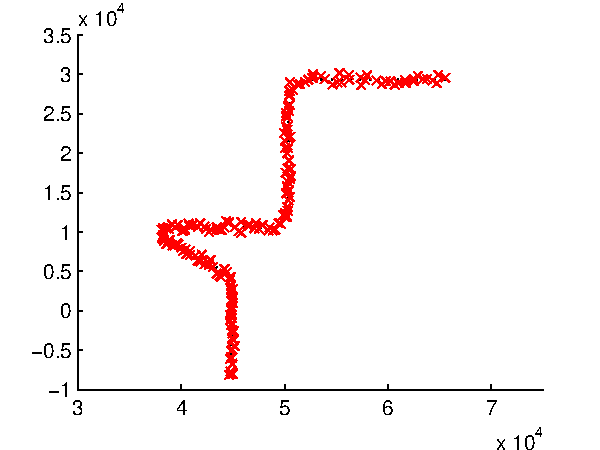
\includegraphics[width=0.95\columnwidth]{images/benchmark_problem.pdf}
\caption{2D benchmark trajectory (dashed) and observations (crosses). Sensor is at (0,0).}
\label{fig:2D_ground_truth}
\end{figure}

All tests were conducted using resample-move steps. 50 filter particles were used for 2D tests and 200 for 3D tests.



\subsection{2D Model with Observed Velocity}

The combination of the basic 2D model and a VRPF has been demonstrated in \cite{Godsill2007} and has been proven effective. However, when the velocity is observed as well as the position (for example using Doppler radar), this can cause the VRPF to produce worse estimates or even to lose track, despite the fact that there is now more information available. This phenomenon is shown in Fig.~\ref{fig:2D_Model1}. By introducing additional drift velocity parameters, the errors are reduced. The result of applying the augmented 2D model to the same problem is shown in Fig.~\ref{fig:2D_Model2}.
%
\begin{figure}[!t]
\centering
\subfloat[Without velocity observations]{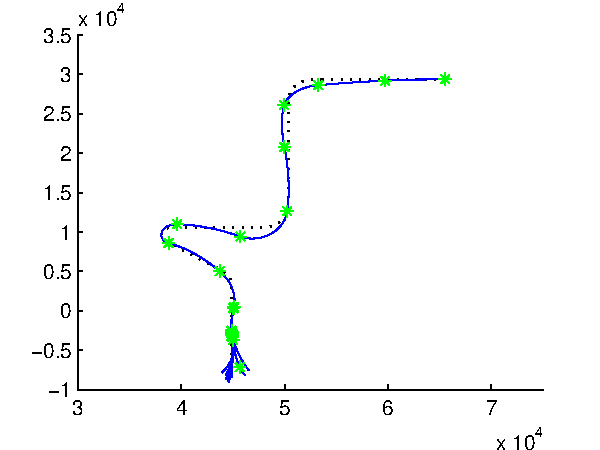
\includegraphics[width=0.95\columnwidth]{images/M1withoutVel.pdf}}
\\
\subfloat[With velocity observations]{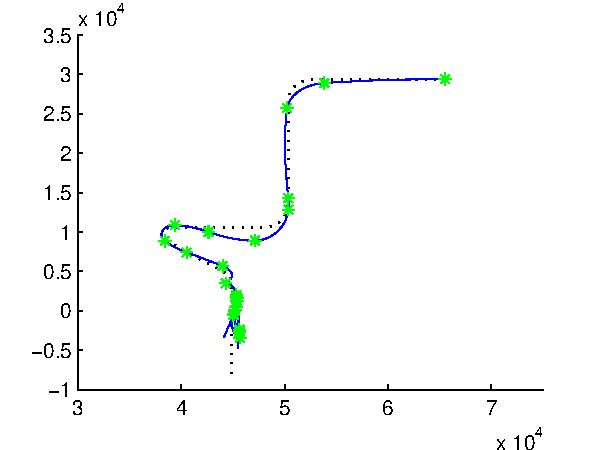
\includegraphics[width=0.95\columnwidth]{images/M1withVel.pdf}}
\caption{Variable rate particle filter results using basic 2D model, with and without range rate observations. Dotted line shows ground truth. Solid lines shown particle estimates. Stars show particle changepoints.}
\label{fig:2D_Model1}
\end{figure}
%
\begin{figure}[!t]
\centering
\subfloat[Without velocity observations]{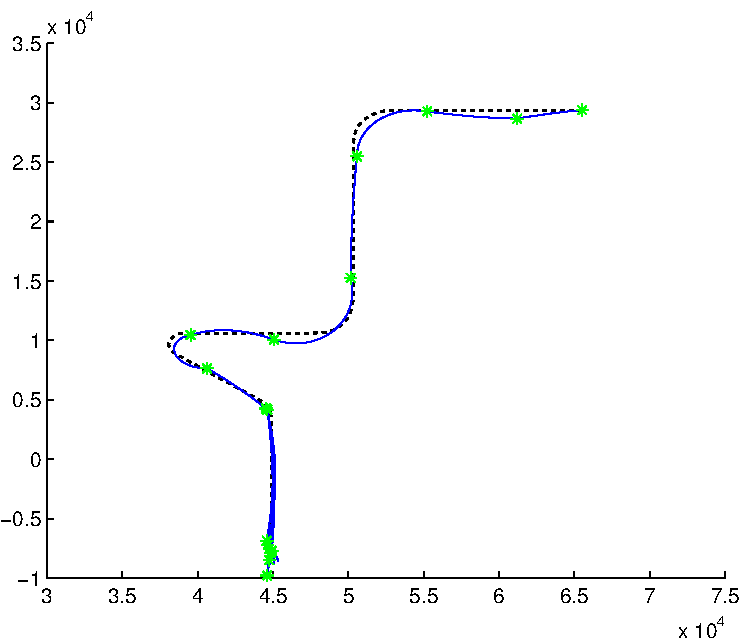
\includegraphics[width=0.95\columnwidth]{images/M2withoutVel.pdf}}
\\
\subfloat[With velocity observations]{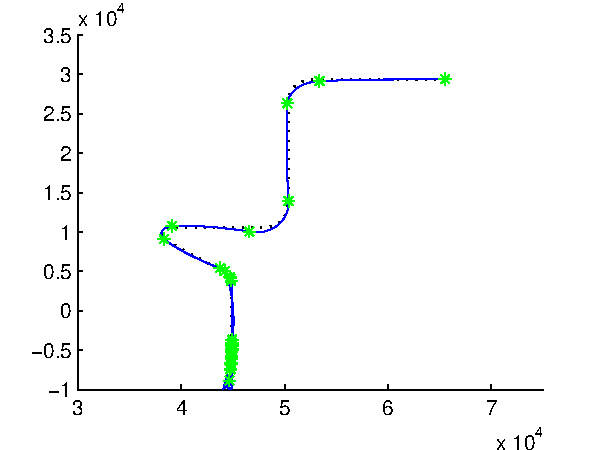
\includegraphics[width=0.95\columnwidth]{images/M2withVel.pdf}}
\caption{Variable rate particle filter results using augmented 2D model, with and without range rate observations. Dotted line shows ground truth. Solid lines shown particle estimates. Stars show particle changepoints.}
\label{fig:2D_Model2}
\end{figure}

The basic and augmented models were tested on 100 realisations of the problem, with and without velocity observations (i.e. using different seeds for the pseudo-random number generator for producing the observations and running the algorithms). The mean error performance in position and velocity is shown in table~\ref{tab:2D_performance}. Two measures of error are compared: one using the filter state estimate (a weighted average of the particle states) and the other a basic smoothing state estimate --- the entire state trajectory is estimated from the final filter approximation, in the similar manner to the filter-smoother of \cite{Kitagawa1996}.
%
\begin{table}
\renewcommand{\arraystretch}{1.3}
\caption{2D VRPF tracking performance with basic and augmented intrinsic coordinate models with and without velocity observations}
\label{tab:2D_performance}
\centering
\begin{tabular}{|c|c|c|c|c|c|}
\hline
      & Observed  & \multicolumn{2}{c|}{Filter RMSEs}  & \multicolumn{2}{c|}{Smoother RMSEs}  \\
Model & Velocity? & Position & Velocity                & Position & Velocity                  \\
      &           & ($m$)    & ($m/s$)                 & ($m$)    & ($m/s$)                   \\
\hline
Basic     & no  & 416 & 129 & 309 & 49 \\
Basic     & yes & 819 & 115 & 695 & 74 \\
\hline
Augmented & no  & 402 & 125 & 220 & 39 \\
Augmented & yes & 705 & 101 & 432 & 43 \\
\hline
\end{tabular}
\end{table}

The augmented model results in a significant reduction in estimation errors, especially when the velocity is observed. However, it does not fully solve the problem of velocity measurements making the estimates less accurate. A solution to this problem will probably require changes to the filtering algorithm. %Note that if the precision of the range rate measurements is increased then track loss becomes more common, and begins to affect the augmented model as well.



\subsection{3D Intrinsic Coordinate Model}

Here we demonstrate the 3D intrinsic coordinate model, and compare it to the Cartesian equivalent used in \cite{Whiteley2007a,Whiteley2011}. The same trajectory is used as before, but this time the altitude components are not discarded. An example realisation is shown in Fig.~\ref{fig:3D_ground_truth}.
%
\begin{figure}
\centering
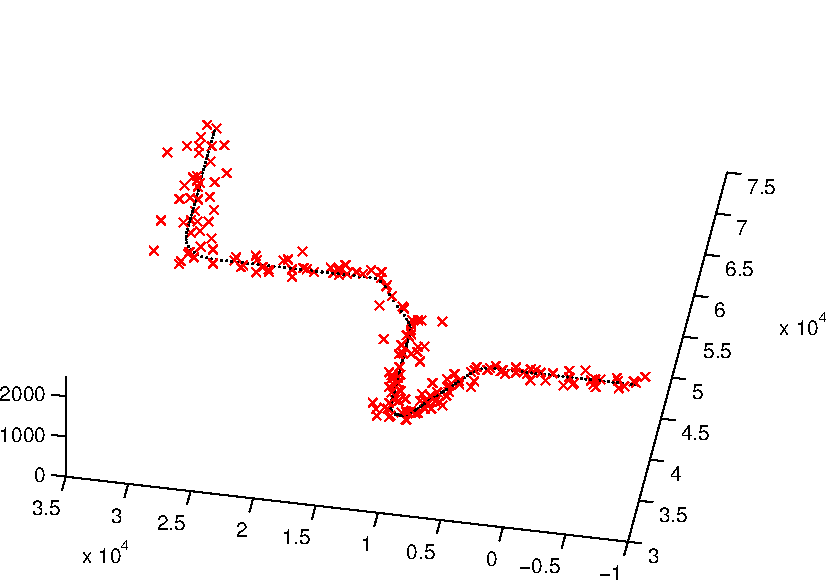
\includegraphics[width=0.95\columnwidth]{images/3Dbenchmark_problem.pdf}
\caption{3D benchmark trajectory (dashed) and observations (crosses). Sensor is at (0,0).}
\label{fig:3D_ground_truth}
\end{figure}

The results of applying the basic 3D intrinsic coordinate and Cartesian models to this data set are show in Fig.~\ref{fig:3D_CartesianIntrinsic}. The intrinsic coordinate model results in better fitting around the corners. Furthermore, the Cartesian model uses more changepoints on average, as the motion is approximated by a larger number of shorter manoeuvres. These improvements can be attributed to the fact that the variance of tangential and normal accelerations can be set independently, accommodating the fact that normal accelerations tend to be much larger.
%
\begin{figure}
\centering
\subfloat[Cartesian]{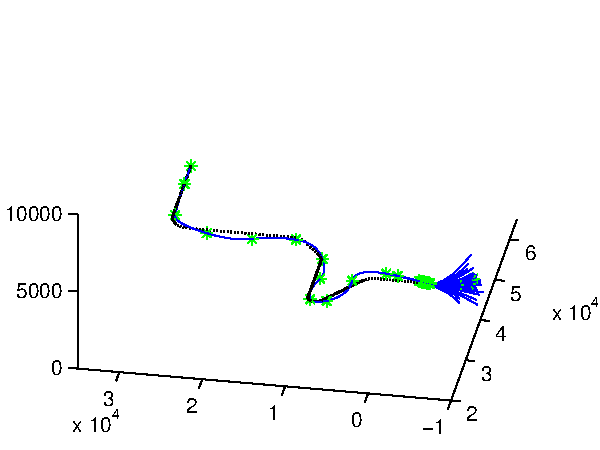
\includegraphics[width=0.95\columnwidth]{images/3DCartesian.pdf}}
\\
\subfloat[Intrinsic]{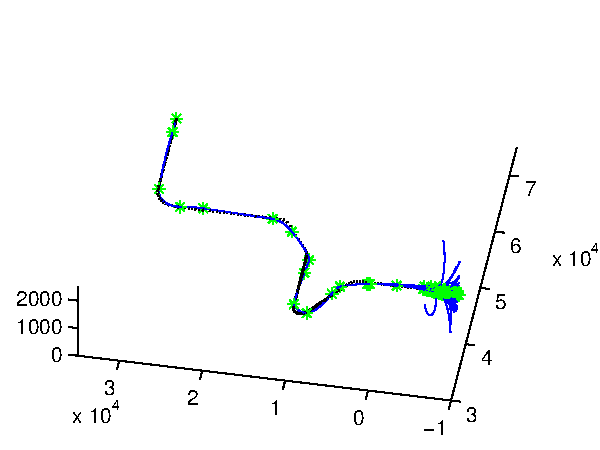
\includegraphics[width=0.95\columnwidth]{images/3DIntrinsic.pdf}}
\caption{Variable rate particle filter results using Cartesian and intrinsic coordinate dynamic models. Dotted line shows ground truth. Solid lines shown particle estimates. Stars show particle changepoints.}
\label{fig:3D_CartesianIntrinsic}
\end{figure}

Testing on 100 realisations, the average error performance is shown in table~\ref{tab:3D_performance}.
%
\begin{table}
\renewcommand{\arraystretch}{1.3}
\caption{3D VRPF tracking performance with basic intrinsic coordinate and Cartesian models}
\label{tab:3D_performance}
\centering
\begin{tabular}{|c|c|c|c|c|c|}
\hline
      & Observed  & \multicolumn{2}{c|}{Filter RMSEs}  & \multicolumn{2}{c|}{Smoother RMSEs}  \\
Model & Velocity? & Position & Velocity                & Position & Velocity                  \\
      &           & ($m$)    & ($m/s$)                 & ($m$)    & ($m/s$)                   \\
\hline
Intrinsic & no  & 401 & 131 & 259 & 43 \\
\hline
Cartesian & no  & 422 & 148 & 291 & 58 \\
\hline
\end{tabular}
\end{table}

The intrinsic coordinate model consistently outperforms the Cartesian version.

These is plenty of scope for improving these models. Clearly, there is more prior information about aircraft in flight which could be incorporated. For example, a predilection for level flight could be quantified through the choice of the distribution of $\phi_k$, the angle of the plane of motion, which is currently uniform.



\section{Conclusion}

Dynamic tracking models for use with variable rate particle filters have been developed. Variable rate models treat the state as a deterministic continuous-time process conditional on a sequence of changepoints and motion parameters. Previously, a system has been developed which models targets as particles moving under the influence of tangential and normal accelerations. These have been developed in two ways. First, additional parameters have been introduced to improve the filter performance when the velocity is observed, for example through the use of Doppler measurements. Second, the model has been extended for use in 3D, where it achieves better state estimation performance than a Cartesian model.



\bibliographystyle{IEEEtran}
\bibliography{D:/pb404/Dropbox/PhD/Cleanbib}

\end{document} 